\chapter{Related Work}
There has been a great deal of research in the areas of Complex Event Processing, Software Defined Networks and High-Performance packet processing. Since this thesis derives motivation from all the three, related work is surveyed and organized according to these domains. In this chapter, the outcomes of the research works and takeaways from the perspective of the thesis are briefly discussed to give the rationale or motivation for the implementation of the thesis.

\section{Deployment Strategies and Operator Placement in Event Processing}
Since the thesis focuses on creating a data plane solution specifically tuned for the Event Processing/Event-Based Systems, it is important that key factors impacting the design of such systems are studied in detail.
Cugola et. al \cite{Cugola} discuss different deployment strategies for distributed complex event processing systems. The strategies described in the paper can be classified based on:
\begin{itemize}
 \item \textbf{Organizing processors into processing trees}: Primitive events from sources are collected, filtered, and processed as the move upwards in the tree. This allows for incremental evaluation at intermediate processors in a manner similar to staged processing. 
 \item \textbf{Forwarding advertisements to processors}: Each processor in the processing tree maintains an advertisement and subscription table.  When receiving an event notification, each processor computes the set of subscriptions that match the event and determine which node in the processing tree receives it. 
 \item \textbf{Rule deployment}: The rules are recursively partitioned into partial rules and deployed in the root to the source of the processing tree. 
 \item \textbf{Notification Forwarding}: Two concepts of event forwarding are discussed - Push-based and Pull based. In Push based forwarding, a processor forwards all matched primitive events to the parent; whereas in Pull based forwarding the processor stores the matched event until it is explicitly asked by the parent. 
\end{itemize}
In addition to deployment strategies, Cugola et. al present an analysis of content-based filtering of primitive events. Their analysis highlights the advantage of content-based filtering close to the source to reduce the network traffic in both distributed and centralized deployment. Their work informs and motivates the thesis at many levels. With a content-aware switch and an SDN-based controller to deploy rules, a logical processing tree based on event types can be constructed to process different event types at different processors.  Since the controller has a logical view of the network, rules can be deployed in such a way that one processing node is responsible for a pre-decided event type. The events from one processing node can be then chained to another based on the logical processing tree using a push based forwarding strategy.\newline 

Pietzuch et. al \cite{pietzuch2006network} discuss the NP-hardness of the operator placement problem and propose a heuristics based approach. They propose a stream based overlay network in between the physical network and the stream processing system and delineate three challenges in the operator placement problem: a) Achieving good application query performance b) Use network efficiently c) Reuse existing operators when appropriate. Zhou et. al \cite{zhou2006efficient} present a cost model for dynamic load balancing in distributed stream processing systems and identify the importance of load balancing in streaming applications. While publications such as \cite{backman2012managing} and \cite{chatzistergiou2014fast} focus on reducing the end to end latency, \cite{aniello2013adaptive} and \cite{cui2016big} focus on reducing the inter-node traffic, and \cite{rizou2010solving}, \cite{pietzuch2006network} focus on reducing the overall network usage. While all the concerns are valid for the distributed event processing environment, the research focuses using the application layer for optimization. Even when an In-Network solution is discussed, the solution is based on deploying processing nodes as close to the data source as possible. The discussed research works provide good motivation for selecting optimization parameters in Event Processing systems. However, the solution provided in the thesis is a data-plane solution, focusing on utilizing the underlying network service instead of the application level processing node.


\section{Fog Computing and Software Defined Internet of Things}
There has been an exponential growth of connected devices, and it is unanimously accepted that the number of connected devices is going to increase from the current 10 billion nodes to 50 billion nodes over the next few years. This presents us with two interesting challenges: 
\begin{itemize}
\item \textbf{Handling massive streams of data from the sensory nodes}: Large cloud deployments of today are designed to handle colossal amounts of data from the web and other batch processing applications. But when there are billions of sensory nodes located in widespread geographic location producing streams of sensor data, transporting all the data to the cloud is counter intuitive. For one, it creates unnecessary traffic in the network because most of the sensing data is discarded anyway and for another, it creates a lot of latency. And as properties of sensory data go, it is mostly useless; but when it is not, it is most likely vital. This problem has been discussed even before the explosion of IoT networks. The operator placement problem discussed in the previous section to some extent attempts to address this problem by moving the operators closer to the sources of data to react to events faster and reduce network traffic. Fog computing is a local cloud deployment paradigm which does exactly this. Bonomi et. al \cite{bonomi2012fog} discuss in detail the characteristics of IoT and advantages of Fog deployment in IoT. 
\item \textbf{Maintaining the massive network for the sensory nodes}: As billions of wired and wireless sensory nodes join the network, traditional networking is insufficient to utilize the paradigm fully. Software Defined Networking which we discussed in Chapter 2.2, introduces significant flexibility for resource management by separating the data plane from a software based control plane. Software Defined Internet of Things promises an architecture to seamless manage, configure, and spawn billions of sensor nodes to create Sensing-as-a-Service(SaaS) paradigm. Research done in \cite{el2015software} , \cite{qin2014software} and \cite{flauzac2015sdn} detail such an architecture and provide prototype deployments with network models.
\end{itemize} 
Truong et. al \cite{truong2015software} deploy a Software defined Fog computing Adhoc vehicular network, whereas Xu et. al \cite{xu2016towards}  prototype a Software Defined Fog computing Message Queueing Telemetry Transport (MQTT) broker for IoT devices. Prototypes built by \cite{xu2016towards} and \cite{flauzac2015sdn} deploy Open vSwitch as the OpenFlow switch in their respective SDN-based Fog deployments. This highlights the versatility of Open vSwitch in both large scale global cloud and small scale local Fog deployments. These works motivate the selection of Open vSwitch for an application-aware deployment in the cloud, be it in large data centers or IoT networks.

\section{Application-aware Data Plane Processing in SDN}
Mekky et. al \cite{mekky2014application} prototype an Application-aware implementation of Open vSwitch(OVS). The prototype implementation, as shown in figure 3.1 - sourced and reinterpreted from \cite{mekky2014application} -  creates a separate application module within the Open v Switch with its own separate app-table. The app-table is staged after the OpenFlow flow table pipeline. The application module is responsible for handling the flow out of the app-table and executing app-actions. An app-action is capable of doing the following operations:
\begin{itemize}
\item Determine actions for a packet and modify the state if required.
\item Generate or modify the rule set for processing this flow.
\item Remove flows from the OpenFlow tables and generate packet out to other switches.
\item Send custom vendor messages to the controller.
\end{itemize}
A table-miss in the standard OpenFlow table is sent to the app-table instead of the controller as in the standard Open vSwitch. The app-table is configurable with custom app-actions. These app-actions are executed within the application module in the userspace. In summary, the application module within the OVS runtime behaves like a light-weight controller capable of receiving select flow, executing them in userspace, and taking decisions by calling the OpenFlow APIs. The research work also provides valuable information about the interception of packets within the OVS as a design choice. Mekky et. al lay out three options to the said end:
\begin{itemize}
 \item Intercept the messages between controller and OVS at the connection manager.
 \item Intercept the packet after looking up the OpenFlow flow table.
 \item Add app-actions directly to flow table and apply actions directly when the rule is matched.
\end{itemize}
 Although the L4-L7 match is supported in the application module, the implementation does not scale to Event Processing paradigms where event patterns can occur in any packet of the stream. In such a scenario, the prototype implementation lifts each packet to the application module and out of the OpenFlow processing pipeline inducing processing latencies. This work provides motivation to keep processing in-line for scenarios such as stream processing where rules have to be applied for each packet in the stream.


 \begin{figure}[H]
 \centering
 \caption{Application Aware Data Plane Processing} 
 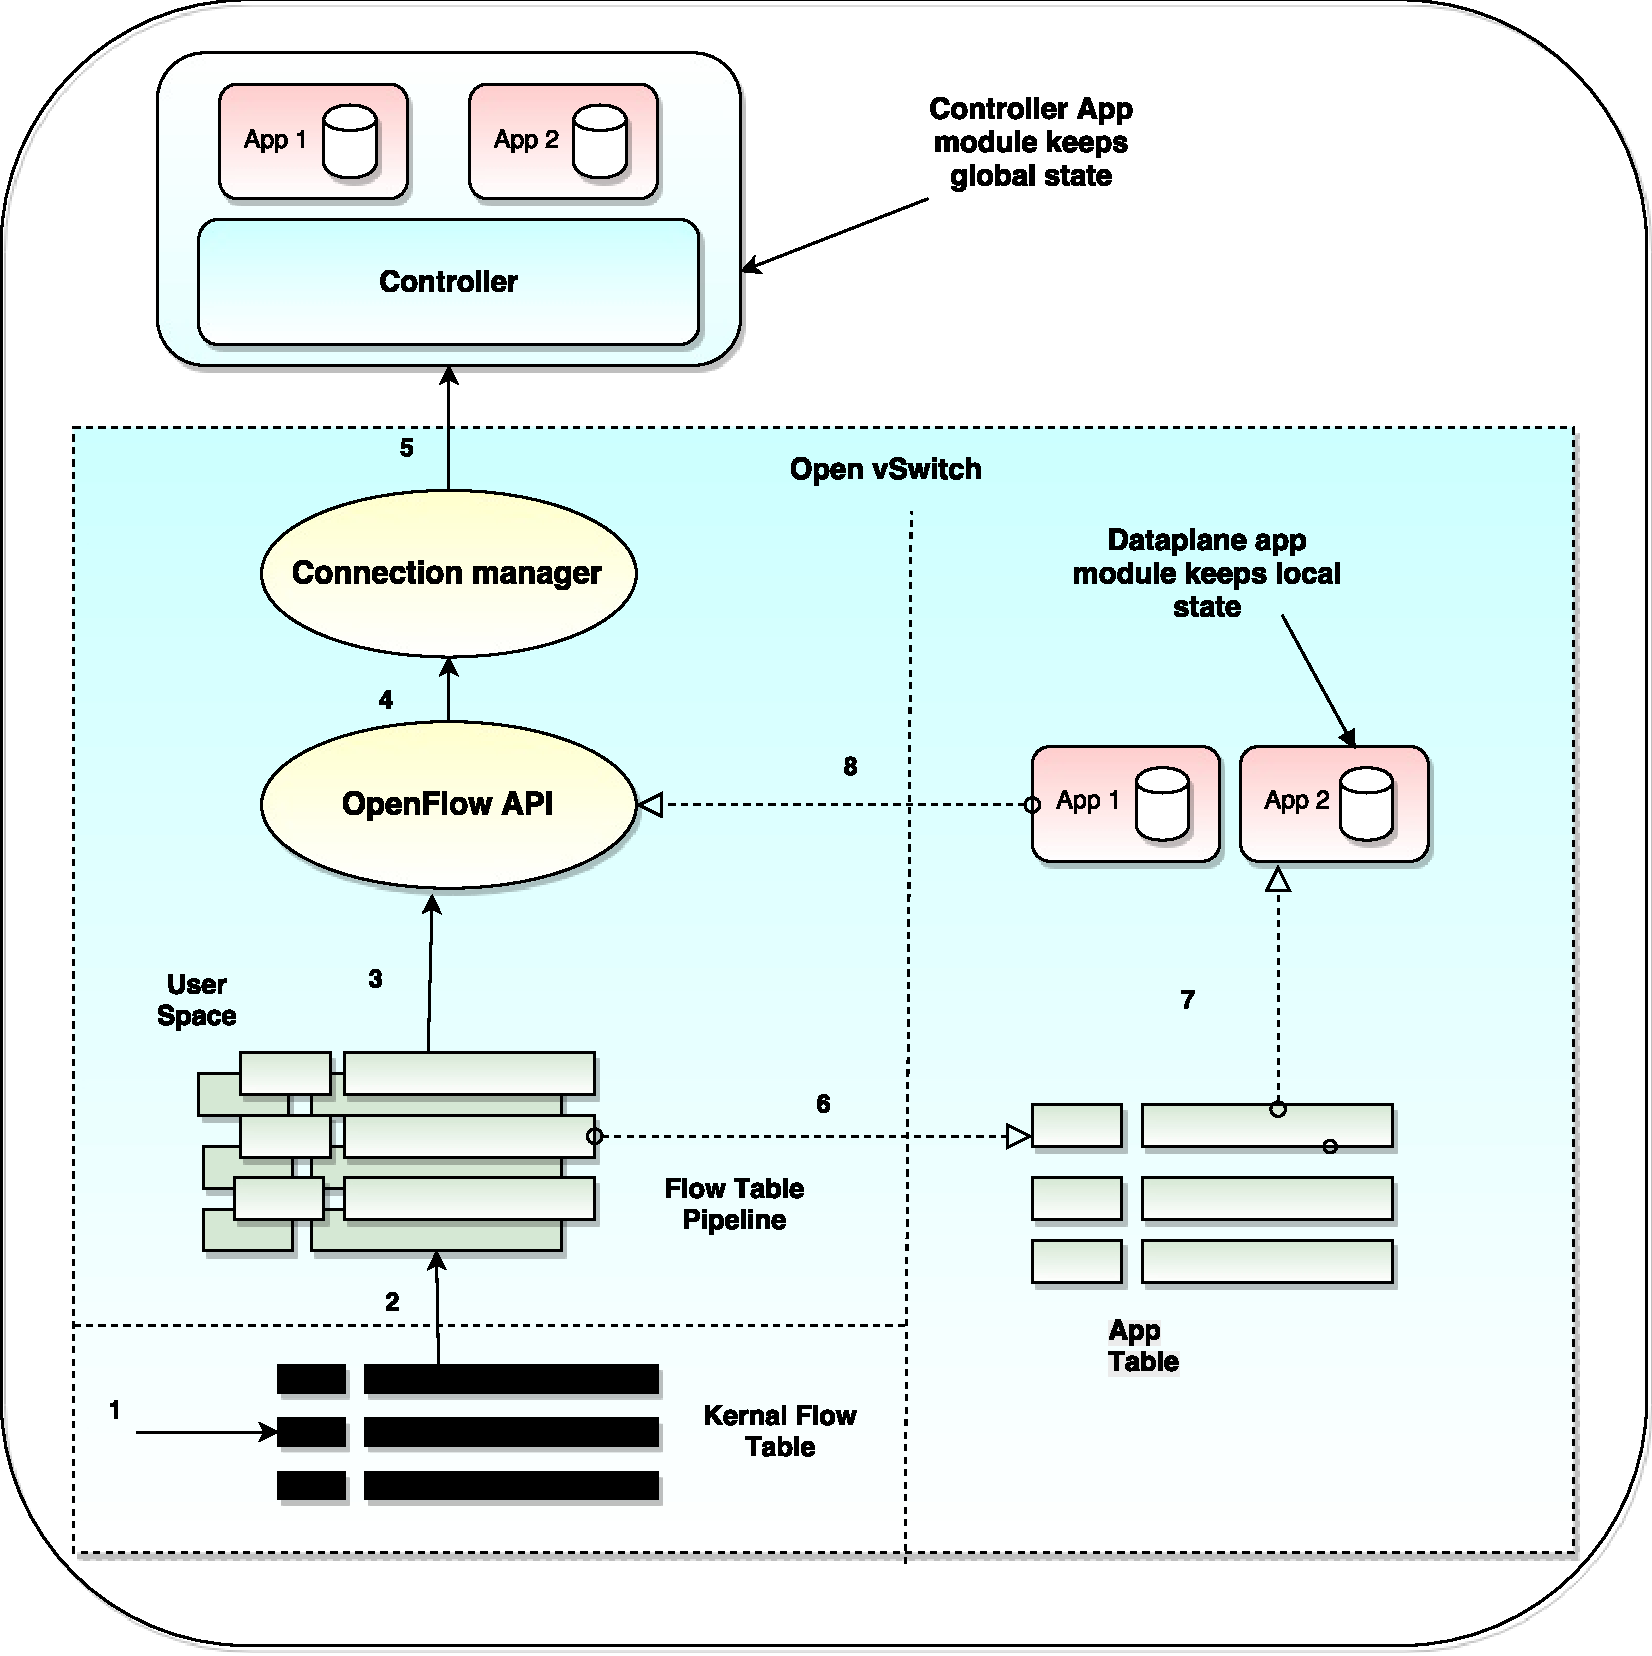
\includegraphics[height=10cm,width=13cm]{appaware01.pdf} 
\end{figure}


\section{In-Net: In-Networking Processing for the Masses}
Stoenescu et. al \cite{NpForMasses} prototype a ClickOS based \cite{martins2014clickos} processing platform running on commodity servers. Their results promise the possibilities of running single, inexpensive commodity servers scattered around in the network with the vision of providing a controller-based access to both network providers and end users. The processing platform, which relies on ClickOS is capable of hosting upwards of thousand clients per box. In this model, end-users can demand adhoc network service, in the box which can be provisioned instantaneously. While they also provide various security configurations and static analysis as a way to measure the validity of the provided service, the deployment model used provides a fascinating insight into the motivation for work done in the thesis. 
In the work done by Martins et. al on ClickOS, they consider two options to for the ClickOS switch

\begin{itemize}
 \item \textbf{VALE based deployment}: The first model uses a modified VALE \cite{Rizzo:2012:VSE:2413176.2413185}, a Virtual Local Ethernet switch to connect the virtual machines. VALE is a software switch which uses netmap (Discussed in Section 2) API and batched packet processing for high performance switching between guest virtual machines.
 \item \textbf{Open vSwitch}: The second model uses a standard Open vSwtich for connecting the guest virtual machines.
\end{itemize}

The results produced, express that the performance of the modified VALE switch is better than that of the standard Open vSwitch; explained partly by VALE's usage of the netmap API - which allows the packet buffers to be mapped to the VM's memory space - and other modified APIs enabling batched packet processing.

 \begin{figure}[H]
 \centering
 \caption{In-Network processing model} 
 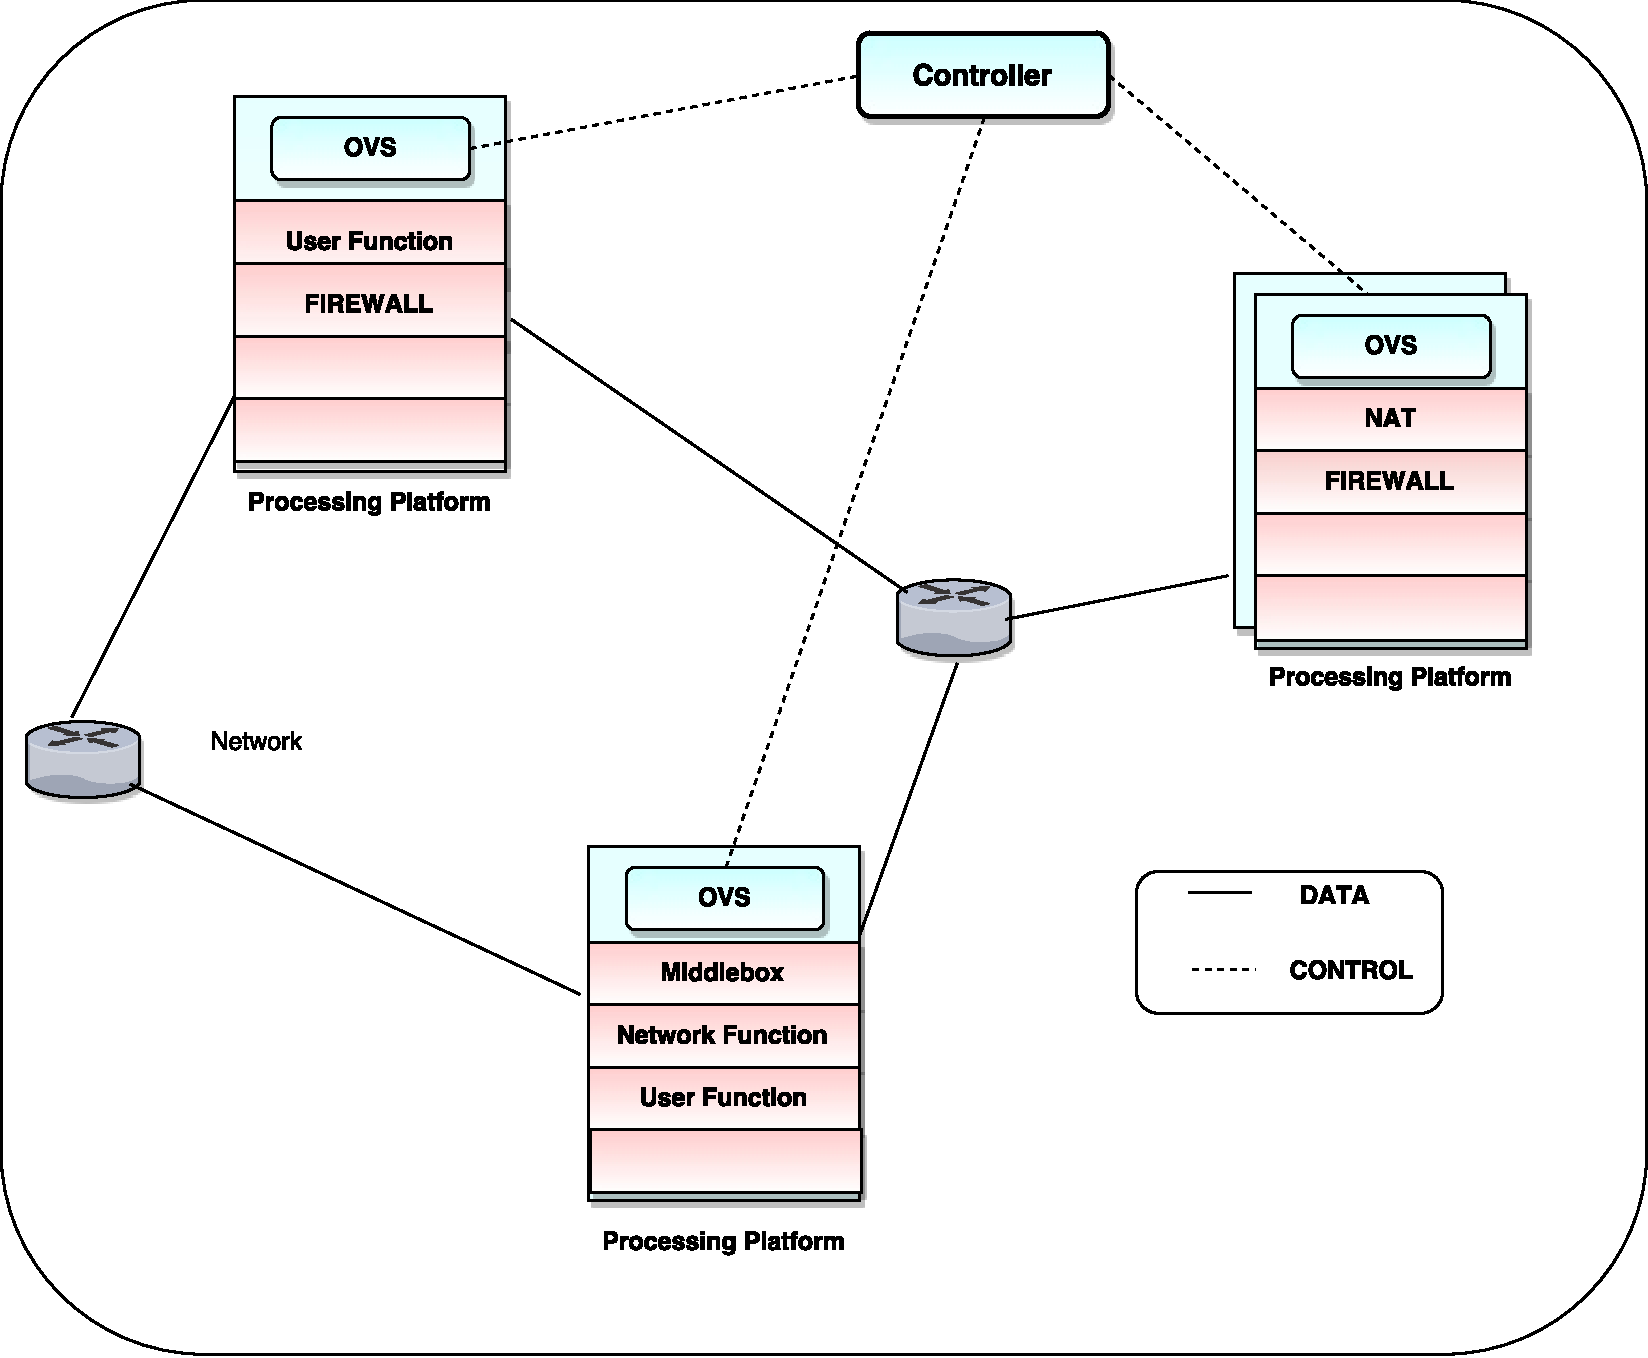
\includegraphics[height=10cm]{innet01.pdf} 
\end{figure}

However, the implementation by Stoenescu et. al \cite{NpForMasses} uses the Open vSwitch within their processing platform, highlighting the versatility of Open vSwitch. The ability of the Open vSwitch to speak OpenFlow and thereby be configured by controllers in the Software Defined Networking model makes it a valuable option for deployment in In-Networking processing scenarios. One such deployment scenario is detailed in figure 3.2 - sourced and reinterpreted from \cite{NpForMasses}. As we can see, the processing platforms are dispersed all around the network. Each processing platform consists of an Open vSwtich which is capable of speaking OpenFlow. The users and network operators rely on the OpenFlow controller to request, provision or service network functions. Although the performance of Open vSwitch does not compare well to that of a hardware unit, its versatility makes it a great design choice. Moreover, with the advent of DPDK, the performance of Open vSwith can be vastly improved, all the more consolidating Open vSwitch as a design choice for the implementation in the thesis.

\section{SmartSwitch: Blurring the Line Between Network Infrastructure and Cloud Applications}
Wei Zhang et. al \cite{zhang2014smartswitch} prototype an application-aware networking platform that performs functions that are characteristically performed by computing platforms. They explore how the boundaries between applications and network infrastructure can be obscured by modern day packet-processing technologies.  They prototype a memcache-aware switch, which achieves application level redirection to memcached servers and local caching to allow immediate responses to hot requests. The paper examines three areas as use cases for their effort:
\begin{itemize}

 \item  \textbf{Load balancing}: Although SDN allows for a much more flexible policy-shaping of the data plane, it still does not allow decision making based on data plane information. The packets still have to be sent to load balancers and proxies for content based routing. An application-aware implementation may try to overcome this problem by enabling the software switch to perform redirection based on the application data.
.
 \item  \textbf{Storing Data within the network}: Focusing on content-centric networks where forwarding requests and responses are based on names rather than location, an application aware switch may be equipped with a Hadoop-aware implementation and populated with cache keys and individual names for the keys. Doing so allows the switch to direct requests to nearest cache locations.

 \item  \textbf{Computation in the network}: When application data has to traverse through multiple Wide Area Networks, Wei Zhang et. al propose that it is more intelligent to process or store only the information that is relevant for the application. To this end, they discuss the ability to deploy computation within the network to process and filter the data instead of blind routing/forwarding at the network. They contrast this with providing hardware based switching which incurs a high cost and is not flexible to changing demands of the application.

\end{itemize}
The Smart switch prototype is implemented along the above lines and is evaluated against Twitter's TwemProxy server. Initial evaluation results show that the Smartswitch significantly reduces the latency for cached data. The work done in this paper provides motivation to continue exploring the possibilities to offload application context into the network and possibly tune the network services for specific applications. With the advent of Network Functions Virtualization and the resulting ad-hoc provisioning of network services in the network pipeline, this paper provides invaluable direction for the thesis. 

\section{NetVM: High Performance and Flexible Network Virtualization}
Hwang et. al \cite{hwang2015netvm} present a high-speed network virtualization platform which promises line speed performance for high bandwidth network functions. They innovate on top of the Linux KVM and Intel DPDK platforms to provide:
\begin{itemize}
 \item A virtualization platform for network service provisioning which can perform at the level of custom hardware packet processing.
 \item A zero-copy delivery mechanism between VM's via their shared-memory framework.
 \item A hypervisor switch for intelligent load balancing via state-dependent or data-dependent approach.
 \item An architecture which enables the compositing of complex network services on multiple VMs.
 \item Security domains that differentiate between trusted and untrusted VM's for packet processing.
\end{itemize}

 \begin{figure}[H]
 \centering
 \caption{NetVM} 
 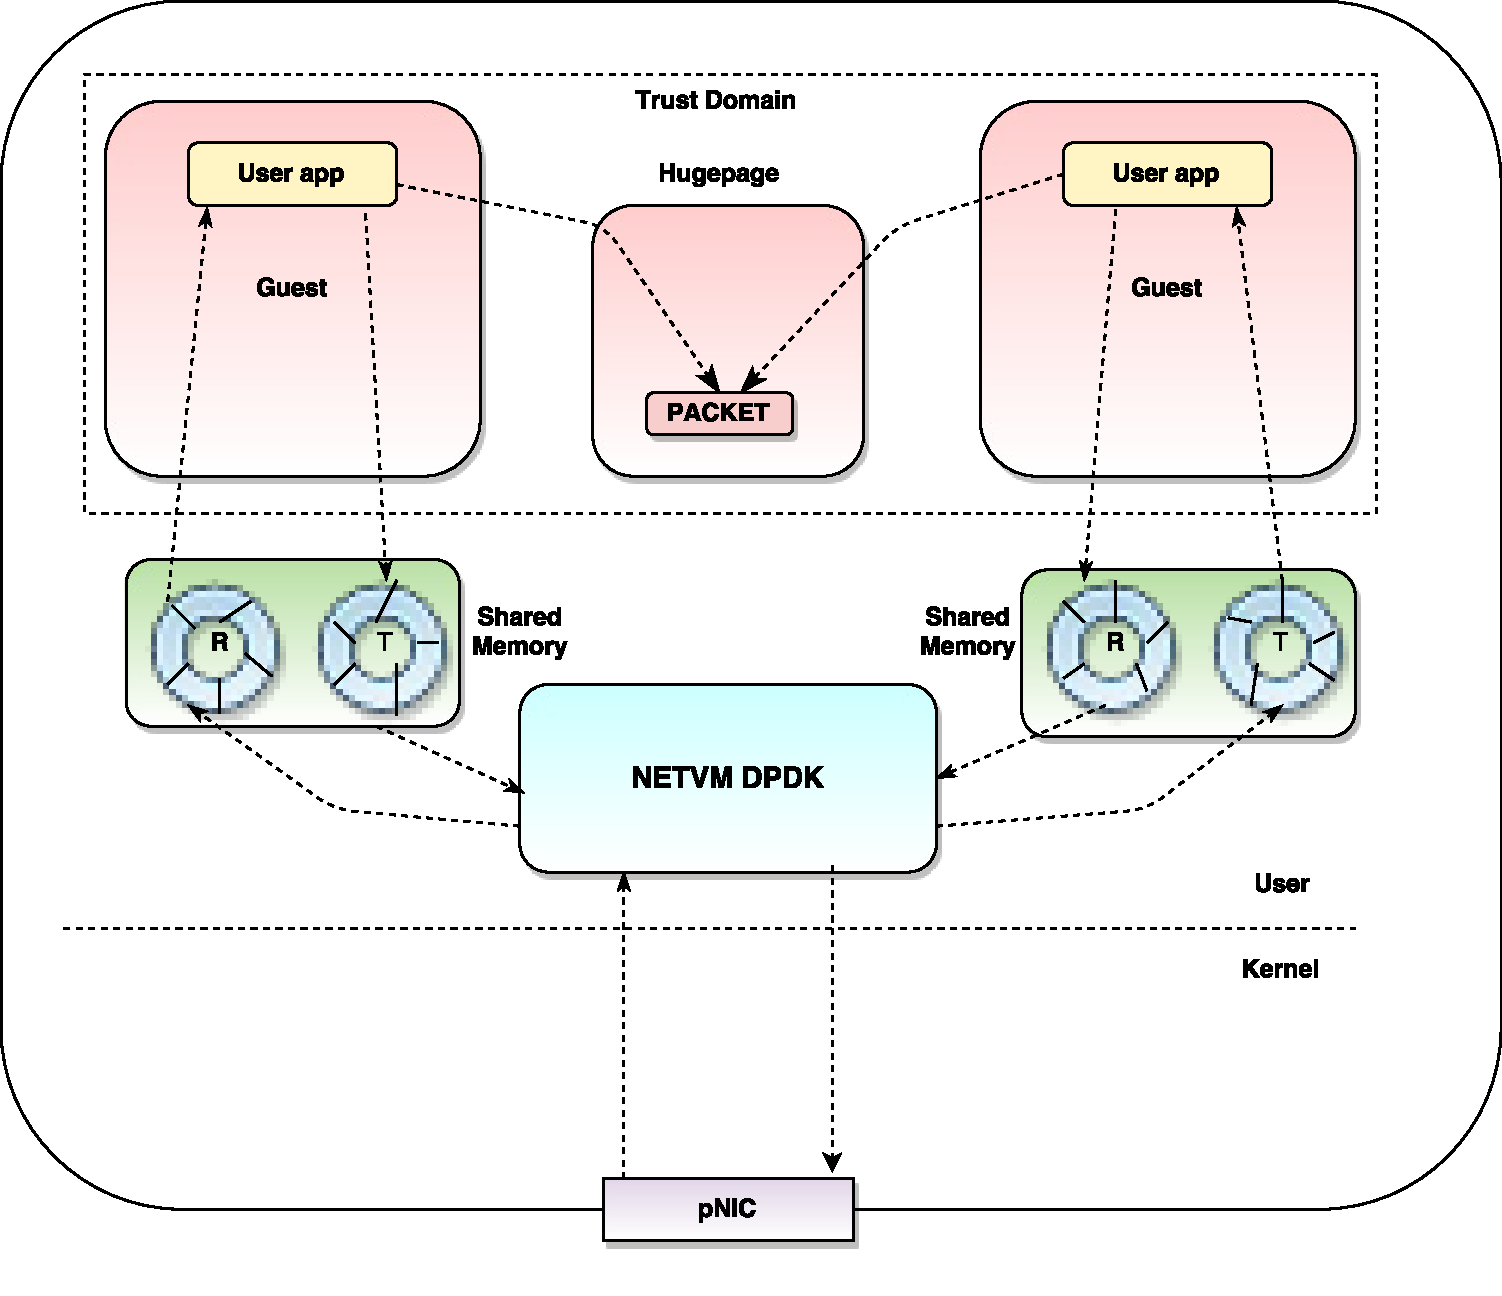
\includegraphics[height=10cm]{netvm01.pdf} 
\end{figure}

\subsection*{Zero-Copy Packet Delivery}
NetVM implements a Hypervisor switch, accelerated by the DPDK library. The implementation leverages DPDK hugepages support (discussed in detail in Chapter 2) and adds its zero-copy framework. As shown in figure 3.3 - sourced and reinterpreted from\cite{hwang2015netvm} - NetVM achieves zero-copy packet delivery by using two strategies: 
\begin{itemize}

\item \textbf{Shared Descriptor Rings}: Shared memory regions are created between the hypervisor and individual guests. This region is used by the guests and the hypervisor switch to descriptors of an incoming or outgoing packet. The packet descriptor contains the location of the packet buffer and also the corresponding action for the packet. As a consequence a packet need not be copied between the hypervisor and the guest; only the packet descriptor is inserted into the corresponding Receive/Transmit descriptor ring within the shared memory location.

\item \textbf{Shared Hugepages}: Hugepages are shared within a group of trusted guests. The DPDK enabled NetVM core polls the Physical NIC and DMA's the packet directly into the hugepage region. Depending on the destination VM for the packet, the NetVM inserts a packet descriptor in the above mentioned shared descriptor ring of the corresponding VM. The VM on receiving the descriptor extracts the packet buffer location in the hugepage area, and directly accesses the packet. Similarly, when a packet has to be transmitted to another guest VM, the sending VM first places the packet descriptor in the descriptor ring. NetVM core extracts packet action from the descriptor and places the packet descriptor in the descriptor ring of the destination VM. The destination VM can now extract the packet buffer location and thereby access the packet without a single copy.
\end{itemize}

Apart from a zero-copy framework, Hwang et. al present other decisions involved during the design of their virtualization platform:


\subsection*{Lockless Design}
Conventionally shared memory locations are managed using locks, which serialize data accesses and increase the overhead involved in communication. A design which uses locks is a huge bottleneck in high-speed networking because of the context switch required to gain and release the locks. Therefore NetVM uses a lockless approach by implementing parallel queues and assigning dedicated cores to service them. At any point, there is only one Producer thread running on a queue, which is run on the hypervisor core, and there is one consumer thread that performs packet processing that is run on the guest VM. Since there is only one producer thread and one consumer thread, there is no need for synchronization. Additionally, even in the case of the shared hugepages, only one guest is ever in control of a packet's descriptor. As an extension, only one application accesses the packet at a given moment ruling out the need for expensive synchronization primitives.
\subsection*{Numa-Aware Design}
In Multi-processor systems cores on different socket accessing the same cache line results in expensive cache invalidation messages. NetVM sidesteps this issue by allocating and using hugepages in a way that each socket has its share of hugepage and the guest threads which access this region of hugepages are pinned to a particular socket. NetVM achieves NUMA-awareness by creating as many Receive/Transmit threads in the hypervisor as there are sockets and each thread is used to process the packets local to that socket. So when the packet is accessed by the host or the guest, it always remains in the local memory. This design creates a pipeline for packet processing such that even when packets traverse from one guest to another, the threads used to process them remain are selected such that there are no cache overheads.
\subsection*{Hugepage Virtual Address Mapping}
Hugepages represent a contiguous memory area to the guests. But because of the NUMA aware design, these hugepages are non-contiguously allocated by the hypervisor. So normally the address of a packet at the hypervisor does not make sense to the guests. And looking up these addresses adds an overhead while performing line-rate packet processing. This challenge is overcome by NetVM by exposing hugepages to the guests using a emulated PCI devices. The guests poll the emulated device and map its memory to userspace. This makes the hugepages appear contiguous to the guest. After this point, NetVM uses a precomputed lookup table and bit operations to convert packet address to a hugepage index and offset.
\subsection*{Trusted and Untrusted Domains}
NetVM creates security domains within a processing host. A virtual machine is assigned to a trust group which decides its access to a range of memory. Virtual machines not given access to a trust group cannot access the hugepage areas allocated to another trust group. Hwang et. al also discuss the possibilities to subdivide security groups such that the DPDK classification engine is used to decide which hugepage pool a packet must be DMA'd into, thereby creating a mechanism to slice flows depending on trust groups.
